\Chapter{Psionics}
{To one extent or another, every human and demi-human on Athas has psionic powers. Most people are wild talents, with only one power that they have learned to use by trial and error. But anyone can harness their psionic powers through careful practice and study, and every city has at least one training hall dedicated to teaching `the way of the mind.' Many warriors, templars, and wizards have attended these academies and developed powerful psionic abilities in addition to their normal talents.}
{The Wanderer's Journal}

\Capitalize{P}{sionic} powers spring from sentient minds. Even an undead creature or a being that has no physical form can create a reserve of inner strength necessary to manifest powers, as long as it has an Intelligence score of at least 1. Vermin possessed of a hive mind ability are an exception to this rule.

A psionic power is a one-time psionic effect. Psionic characters and creatures need not prepare their powers for use ahead of time. They either have sufficient power points to manifest a power or they do not.

A power is manifested when a psionic character pays its power point cost. Some psionic creatures automatically manifest powers, called psi-like abilities, without paying a power point cost. Other creatures pay power points to manifest their powers, just as characters do.

Each power has a specific effect. A power known to a psionic character can be used whenever he or she has power points to pay for it.

\begin{figure*}[b!]
\centering
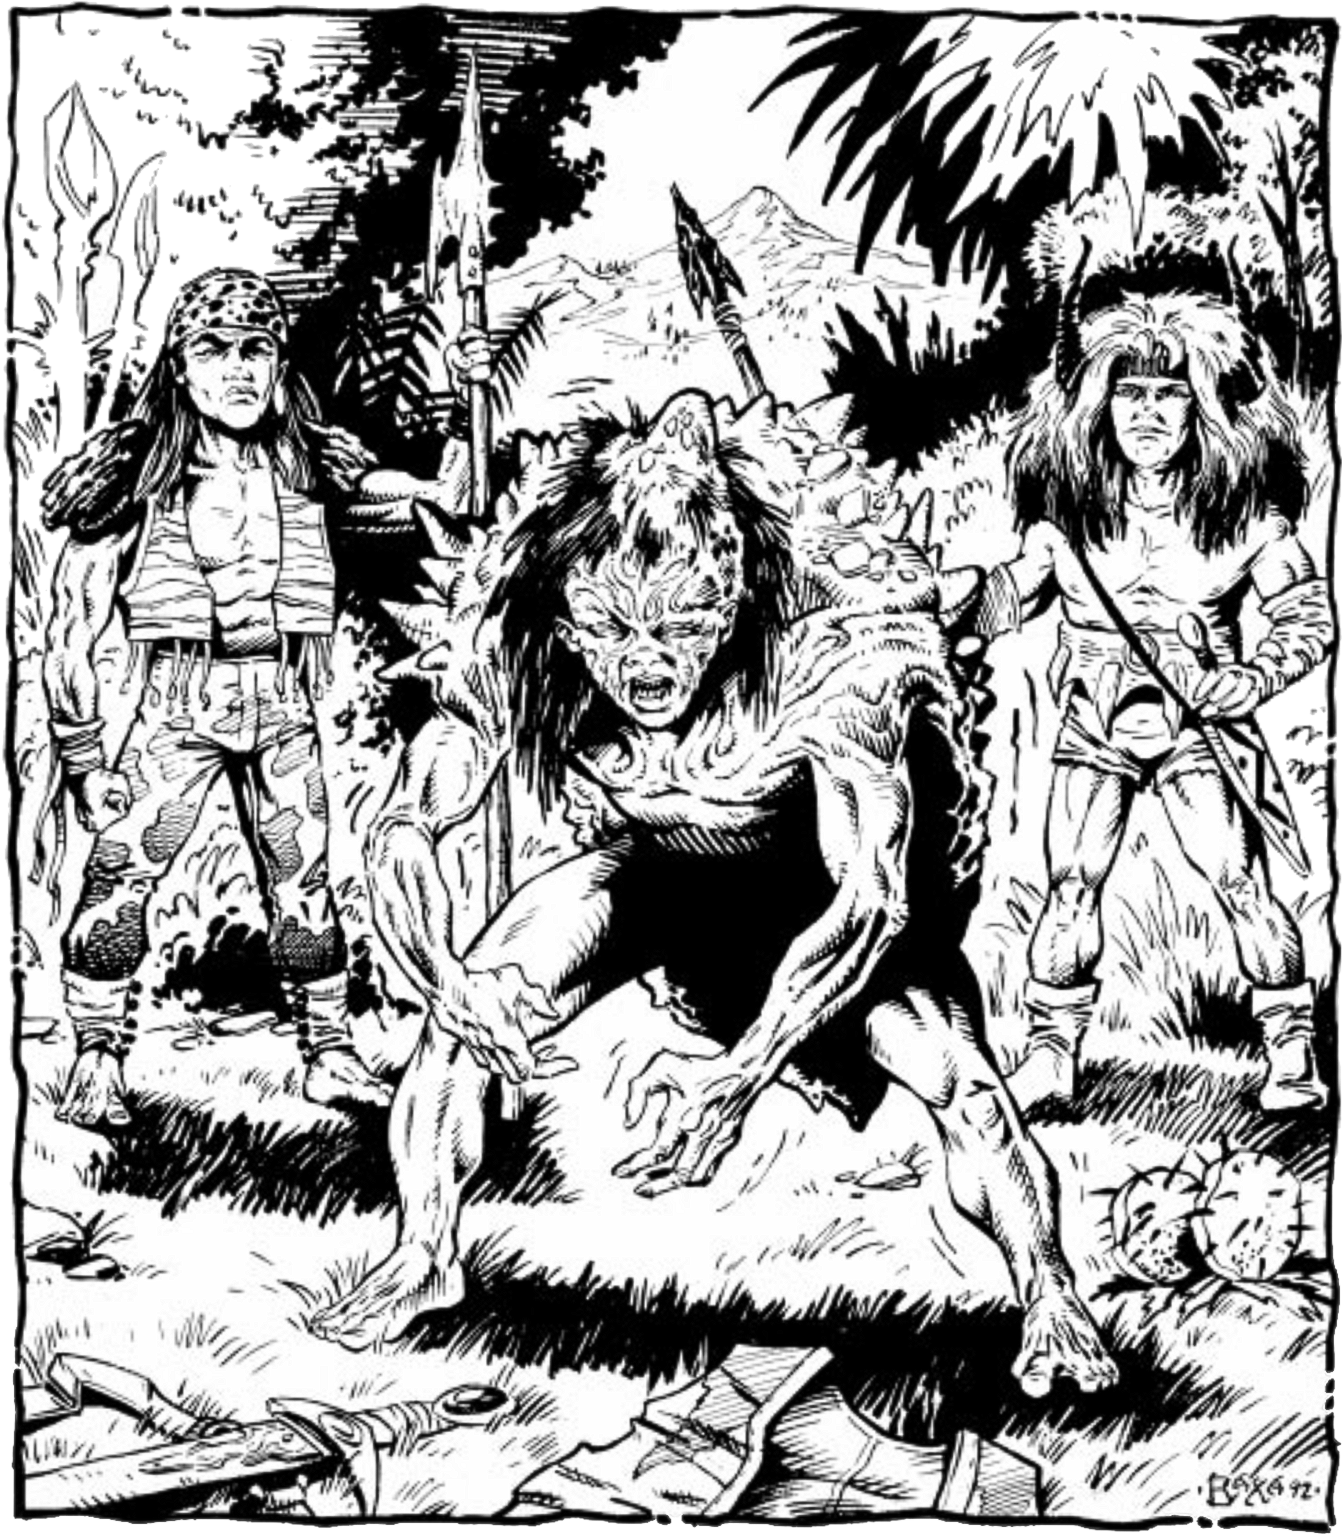
\includegraphics[width=\textwidth-2cm]{images/psionic-2.png}
\par\textit{\small\textcopyright Wizards of the Coast, 2020.}
\end{figure*}

\section{Manifesting Powers}
Psionic characters and creatures manifest powers. Whether they cost power points when manifest by a psionic character, or are manifested as psi-like abilities, powers' effects remain the same. The process of manifesting a power is akin to casting a spell, but with significant differences.

\subsection{Choosing A Power}
First you must choose which power to manifest. You can select any power you know, provided you are capable of manifesting powers of that level or higher. To manifest a power, you must pay power points, which count against your daily total. You can manifest the same power multiple times if you have points left to pay for it.

\subsection{Concentration}
To manifest a power, you must concentrate. If something threatens to interrupt your concentration while you're manifesting a power, you must succeed on a \skill{Concentration} check or lose the power points without manifesting the power. The more distracting the interruption and the higher the level of the power that you are trying to manifest, the higher the DC. (Higher-level powers require more mental effort.)

\textbf{Injury:} Getting hurt or being affected by hostile psionics while trying to manifest a power can break your concentration and ruin a power. If you take damage while trying to manifest a power, you must make a \skill{Concentration} check (DC 10 + points of damage taken + the level of the power you're manifesting). The interrupting event strikes during manifestation if it occurs between when you start and when you complete manifesting a power (for a power with a manifesting time of 1 round or longer) or if it comes in response to your manifesting the power (such as an attack of opportunity provoked by the manifesting of the power or a contingent attack from a readied action).

If you are taking continuous damage half the damage is considered to take place while you are manifesting a power. You must make a \skill{Concentration} check (DC 10 + \onehalf the damage that the continuous source last dealt + the level of the power you're manifesting).

If the last damage dealt was the last damage that the effect could deal then the damage is over, and it does not distract you.

Repeated damage does not count as continuous damage.

\textbf{Power:} If you are affected by a power while attempting to manifest a power of your own, you must make a \skill{Concentration} check or lose the power you are manifesting. If the power affecting you deals damage, the \skill{Concentration} DC is 10 + points of damage + the level of the power you're manifesting. If the power interferes with you or distracts you in some other way, the \skill{Concentration} DC is the power's save DC + the level of the power you're manifesting. For a power with no saving throw, it's the DC that the power's saving throw would have if a save were allowed.

\textbf{Grappling or Pinned:} To manifest a power while grappling or pinned, you must make a \skill{Concentration} check (DC 20 + the level of the power you're manifesting) or lose the power.

\textbf{Vigorous Motion:} If you are riding on a moving mount, taking a bouncy ride in a wagon, on a small boat in rough water, belowdecks in a storm-tossed ship, or simply being jostled in a similar fashion, you must make a \skill{Concentration} check (DC 10 + the level of the power you're manifesting) or lose the power.

\textbf{Violent Motion:} If you are on a galloping horse, taking a very rough ride in a wagon, on a small boat in rapids or in a storm, on deck in a storm-tossed ship, or being tossed roughly about in a similar fashion, you must make a \skill{Concentration} check (DC 15 + the level of the power you're manifesting) or lose the power.

\textbf{Violent Weather:} If you are in a high wind carrying blinding rain or sleet, the DC is 5 + the level of the power you're manifesting. If you are in wind-driven hail, dust, or debris, the DC is 10 + the level of the power you're manifesting. In either case, you lose the power if you fail the \skill{Concentration} check. If the weather is caused by a power, use the rules in the Power subsection above.

\textbf{Manifesting Powers on the Defensive:} If you want to manifest a power without provoking attacks of opportunity, you need to dodge and weave. You must make a \skill{Concentration} check (DC 15 + the level of the power you're manifesting) to succeed. You lose the power points without successful manifestation if you fail.

\textbf{Entangled:} If you want to manifest a power while entangled in a net or while affected by a power with similar effects you must make a DC 15 \skill{Concentration} check to manifest the power. You lose the power if you fail.
\subsection{Power Check}
You must make a special ability check to manifest your chosen power:

\begin{Formula}{1d20 + \textit{key ability score}}
	\item Difficulty Class = 20 + \textit{power level}
\end{Formula}

\textit{Note:} The check adds the ability score, not the ability modifier.

The key ability depends on the discipline of the power being manifested. See \tabref{Disciplines and Associated Abilities}.

\Table{Disciplines and Associated Abilities}{XX}{
\tableheader Discipline & \tableheader Associated Ability \\
Psychometabolism & Constitution \\
Psychoportation  & Constitution \\
Psychokinesis    & Intelligence \\
Metacreativity   & Intelligence \\
Clairscience     & Wisdom \\
Telepathy        & Wisdom \\
}

\textbf{Failure:} If you fail your power check, you lose half of the power points without manifesting the power.

\subsection{Manifester Level}
The variables of a power's effect often depend on its manifester level, which is equal to your psionic class level. A power that can be augmented for additional effect is also limited by your manifester level (you can't spend more power points on a power than your manifester level). See Augment under Descriptive Text, below.

You can manifest a power at a lower manifester level than normal, but the manifester level must be high enough for you to manifest the power in question, and all level-dependent features must be based on the same manifester level.

In the event that a class feature or other special ability provides an adjustment to your manifester level, this adjustment applies not only to all effects based on manifester level (such as range, duration, and augmentation potential) but also to your manifester level check to overcome your target's power resistance and to the manifester level used in dispel checks (both the dispel check and the DC of the check).

\subsection{Power Failure}
If you try to manifest a power in conditions where the characteristics of the power (range, area, and so on) cannot be made to conform, the manifestation fails and half of the power points are wasted.

Powers also fail if your power check fails (see Power Check, above), or if your concentration is broken (see Concentration, above).

\subsection{The Power's Result}
Once you know which creatures (or objects or areas) are affected, and whether those creatures have made successful saving throws (if any were allowed), you can apply whatever results a power entails.

\subsection{Special Power Effects}
Certain special features apply to all powers.

\textbf{Attacks:} Some powers refer to attacking. All offensive combat actions, even those that don't damage opponents, such as disarm and bull rush, are considered attacks. All powers that opponents can resist with saving throws, that deal damage, or that otherwise harm or hamper subjects are considered attacks. Astral construct and similar powers are not considered attacks because the powers themselves don't harm anyone.

\textbf{Bonus Types:} Many powers give creatures bonuses to ability scores, Armor Class, attacks, and other attributes. Each bonus has a type that indicates how the power grants the bonus. The important aspect of bonus types is that two bonuses of the same type don't generally stack. With the exception of dodge bonuses, most circumstance bonuses, and racial bonuses, only the better bonus works (see Combining Psionic and Magical Effects, below). The same principle applies to penalties---a character taking two or more penalties of the same type applies only the worst one.

\textbf{Bringing Back the Dead:} Various psionic powers, such as reality revision and psionic revivify, have the ability to restore slain characters to life. When a living creature dies, its soul departs the body, leaves the Material Plane, travels through the Astral Plane, and goes to abide on the plane where the creature's deity resides. If the creature did not worship a deity, its soul departs to the plane corresponding to its alignment. Bringing someone back from the dead means retrieving his or her soul and returning it to his or her body.

\textit{Level Loss:} The passage from life to death and back again is a wrenching journey for a being's soul. Consequently, any creature brought back to life usually loses one level of experience. The character's new experience point total is midway between the minimum needed for his or her new (reduced) level and the minimum needed for the next one. If the character was 1st level at the time of death, he or she loses 2 points of Constitution instead of losing a level. This level loss or Constitution loss cannot be repaired by any mortal means, even the spells wish or miracle. A revived character can regain a lost level by earning XP through further adventuring. A revived character who was 1st level at the time of death can regain lost points of Constitution by improving his or her Constitution score when he or she attains a level that allows an ability score increase.

\textit{Preventing Revivification:} Enemies can take steps to make it more difficult for a character to be returned from the dead. Keeping the body prevents others from using a single manifestation of reality revision to restore the slain character to life.

\textit{Revivification Against One's Will:} A soul cannot be returned to life if it does not wish to be. A soul knows the name, alignment, and patron deity (if any) of the character attempting to revive it and may refuse to return on that basis.
\subsection{Combining Psionic And Magical Effects}
Athasian magic works in a very different way than psionics and most forms of protection do not apply to both.

\textbf{Psionics-Magic Dissonance}: Magic and psionics are two very different sources of power that don't speak to each other. This creates a complex relationship between them.

\textit{Dispel}: The \spell{dispel magic} spell has no effect against psionic powers, abilities, or items. At the same time, the \psionic{dispel psionics} power has no effect against spells, spell-like abilities, or magic items.

\textit{Power Resistance and Spell Resistance}: Likewise, psionic powers are unimpeded by spell resistance, and spells are not affected by power resistance.

\textit{Antimagic and Null Psionics}: The \spell{antimagic field} does not block psionics, and \psionic{null psionics field} does not suppress magic.

\textbf{Multiple Effects}: Powers or psionic effects usually work as described no matter how many other powers, psionic effects, spells, or magical effects happen to be operating in the same area or on the same recipient. Except in special cases, a power does not affect the way another power or spell operates. Whenever a power has a specific effect on other powers or spells, the power description explains the effect (and vice versa for spells that affect powers). Several other general rules apply when powers, spells, magical effects, or psionic effects operate in the same place.

\textbf{Stacking Effects}: Powers that provide bonuses or penalties on attack rolls, damage rolls, saving throws, and other attributes usually do not stack with themselves. More generally, two bonuses of the same type don't stack even if they come from different powers, or one from a power and one from a spell. You use whichever bonus gives you the better result.

\textit{Different Bonus Types}: The bonuses or penalties from two different powers, or a power and a spell, stack if the effects are of different types. A bonus that isn't named (just a ``+2 bonus'' rather than a ``+2 insight bonus'') stacks with any bonus.

\textit{Same Effect More than Once in Different Strengths}: In cases when two or more similar or identical effects are operating in the same area or on the same target, but at different strengths, only the best one applies. If one power or spell is dispelled or its duration runs out, the other power or spell remains in effect (assuming its duration has not yet expired).

\textit{Same Effect with Differing Results}: The same power or spell can sometimes produce varying effects if applied to the same recipient more than once. The last effect in a series trumps the others. None of the previous spells or powers are actually removed or dispelled, but their effects become irrelevant while the final spell or power in the series lasts.

\textit{One Effect Makes Another Irrelevant}: Sometimes, a power can render another power irrelevant.

\textit{Multiple Mental Control Effects}: Sometimes psionic or magical effects that establish mental control render one another irrelevant. Mental controls that don't remove the recipient's ability to act usually do not interfere with one another, though one may modify another. If a creature is under the control of two or more creatures, it tends to obey each to the best of its ability, and to the extent of the control each effect allows. If the controlled creature receives conflicting orders simultaneously, the competing controllers must make opposed Charisma checks to determine which one the creature obeys.

\textbf{Powers and Spells with Opposite Effects}: Powers and spells with opposite effects apply normally, with all bonuses, penalties, or changes accruing in the order that they apply. Some powers and spells negate or counter each other. This is a special effect that is noted in a power's or spell's description.

\textbf{Instantaneous Effects}: Two or more magical or psionic effects with instantaneous durations work cumulatively when they affect the same object, place, or creature.
\section{Powers and Power Points}
Psionic characters manifest powers, which involve the direct manipulation of personal mental energy. These manipulations require natural talent and personal meditation. A psionic character's level limits the number of power points available to manifest powers. A psionic character's relevant high score might allow him to gain extra power points. He can manifest the same power more than once, but each manifestation subtracts power points from his daily limit. Manifesting a power is an arduous mental task. To do so, a psionic character must have a key ability score of at least 10 + the power's level.

\subsection{Recovering Power Points}
Psionic characters have the following ways of recovering power points: sleeping for at least 8 hours, meditating (see \skill{Autohypnosis} skill), and simply resting.

\textbf{Peaceful Environment:} To regain power points, a psionic character must have enough peace, quiet, and comfort to allow for proper concentration. The psionic character's surroundings need not be luxurious, but they must be free from overt distractions, such as combat raging nearby or other loud noises. Exposure to inclement weather prevents the necessary concentration, as does any injury or failed saving throw the character might incur while concentrating on regaining power points.

\textbf{Death and Power Points:} If a character dies, all daily power points stored in his mind are wiped away. A potent effect (such as \psionic{reality revision}) can recover the lost power points when it recovers the character.

\subsubsection{Sleep}
To regain used daily power points, a psionic character must have a clear mind. To clear his mind, he must first sleep for 8 hours. The character does not have to slumber for every minute of the time, but he must refrain from movement, combat, manifesting powers, skill use, conversation, or any other demanding physical or mental task during the rest period. If his rest is interrupted, each interruption adds 1 hour to the total amount of time he has to rest to clear his mind, and he must have at least 1 hour of rest immediately prior to regaining lost power points. If the character does not need to sleep for some reason, he still must have 8 hours of restful calm before regaining power points.

\textbf{Regaining Power Points:} Once the character has rested in a suitable environment, it takes only an act of concentration spanning 1 full round to regain all power points of the psionic character's daily limit.

\textbf{Recent Manifesting Limit/Rest Interruptions:} If a psionic character has manifested powers recently, the drain on his resources reduces his capacity to regain power points. When he regains power points for the coming day, all power points he has used within the last 8 hours count against his daily limit.

\subsubsection{Rejuvenate}
Using the \skill{Autohypnosis} skill, a psionic character can enter a deep state of meditation. Unlike sleep, every hour a psionic character spends rejuvenating recovers power points. A successful \skill{Autohypnosis} DC 20 check allows a psionic character to recover a number of power points equal to their manifester level + 2 per hour. For every 5 point by which the check result exceeds 20, they can recover an additional power point per hour. A psionic character can end this state at any time without any penalty.

\subsubsection{Rest}
When simply resting in a peaceful environment, a psionic character can still recover power points, but at a rate of 2 power points per hour.

\subsection{Adding Powers}
Psionic characters can learn new powers when they attain a new level. A psion can learn any power from the psion list and powers from his chosen disciplines' list. %A wilder can learn any power from the psion/wilder list. A psychic warrior can learn any power from the psychic warrior list.

\textbf{Powers Gained at a New Level:} Psions and other psionic characters perform a certain amount of personal meditation between adventures in an attempt to unlock latent mental abilities. Each time a psionic character attains a new level, they learn additional powers according to their class description. Psions learn new powers of their choice in this fashion. These powers represent abilities unlocked from latency. The powers must be of levels the characters can manifest.
% \textbf{Powers Gained at a New Level:} Psions and other psionic characters perform a certain amount of personal meditation between adventures in an attempt to unlock latent mental abilities. Each time a psionic character attains a new level, he or she learns additional powers according to his class description. Psions, psychic warriors, and wilders learn new powers of their choice in this fashion. These powers represent abilities unlocked from latency. The powers must be of levels the characters can manifest.

\textbf{Independent Research:} A psion also can research a power independently, duplicating an existing power or creating an entirely new one. If characters are allowed to develop new powers, use these guidelines to handle the situation.

Any kind of manifester can create a new power. The research involved requires access to a retreat conducive to uninterrupted meditation. Research involves an expenditure of 200 XP per week and takes one week per level of the power. At the end of that time, the character makes a \skill{Psicraft} check (DC 10 + spell level). If that check succeeds, the character learns the new power if her research produced a viable power. If the check fails, the character must go through the research process again if she wants to keep trying.

\Figure{t}{images/psionic-6.png}
\subsubsection{Manifest an Unknown Power from Another's Powers Known}
A psionic character can attempt to manifest a power from a source other than his own knowledge (usually a power stone or another willing psionic character). To do so, the character must first make contact (a process similar to addressing a power stone, requiring a \skill{Psicraft} check against a DC of 15 + the highest level power in the power stone or repertoire). A psionic character can make contact with only a willing psionic character or creature (unconscious creatures are considered willing, but not psionic characters under the effects of other immobilizing conditions). Characters who can't use power stones for any reason are also banned from attempting to manifest powers from the knowledge of other psionic characters. Mental contact requires 1 full round of physical contact, which can provoke attacks of opportunity. Once contact is achieved, the character becomes aware of all the powers stored in the power stone or all the powers the other character knows up to the highest level of power the contactor knows himself.

Next, the psionic character must choose one of the powers and make a second \skill{Psicraft} check (DC 15 + the power's level) to see if he understands it. If the power is not on his class list, he automatically fails this check.

Upon successfully making contact with another willing psionic character or creature and learning what he can of one power in particular, the character can immediately attempt to manifest that power even if he doesn't know it (and assuming he has power points left for the day). He can attempt to manifest the power normally on his next turn, and he succeeds if he makes one additional \skill{Psicraft} check (DC 15 + the power's level). He retains the ability to manifest the selected power for only 1 round. If he doesn't manifest the power, fails the \skill{Psicraft} check, or manifests a different power, he loses his chance to manifest that power for the day.

\subsection{Using Stored Power Points}
A variety of psionic items exist to store power points for later use, in particular a storage device called a cognizance crystal. Regardless of what sort of item stores the power points, all psionic characters must follow strict rules when tapping stored power points.

\textbf{A Single Source:} When using power points from a storage item to manifest a power, a psionic character may not pay the power's cost with power points from more than one source. He must either use an item, his own power point reserve, or some other discrete power point source to pay the manifestation cost.

\textbf{Recharging:} Most power point storage devices allow psionic characters to ``recharge'' the item with their own power points. Doing this depletes the character's power point reserve on a 1-for-1 basis as if he had manifested a power; however, those power points remain indefinitely stored. The opposite is not true---psionic characters may not use power points stored in a storage item to replenish their own power point reserves.


\section{Power Descriptions}
The description of each power is presented in a standard format. Each category of information is explained and defined below.

\subsection{Name}
The first line of every power description gives the name by which the power is generally known. A power might be known by other names in some locales, and specific manifesters might have names of their own for their powers.

\subsection{Discipline (Subdiscipline)}
Beneath the power name is a line giving the discipline (and the subdiscipline in parentheses, if appropriate) that the power belongs to.

Every power is associated with one of six disciplines. A discipline is a group of related powers that work in similar ways. Each of the disciplines is discussed below.

\subsubsection{Clairsentience}
Clairsentience powers enable you to learn secrets long forgotten, to glimpse the immediate future and predict the far future, to find hidden objects, and to know what is normally unknowable.

For the purpose of psionics-magic transparency, clairsentience powers are equivalent to powers of the divination school (thus, creatures immune to divination spells are also immune to clairsentience powers).

Many clairsentience powers have cone-shaped areas. These move with you and extend in the direction you look. The cone defines the area that you can sweep each round. If you study the same area for multiple rounds, you can often gain additional information, as noted in the descriptive text for the power.

\textbf{Scrying:} A power of the scrying subdiscipline creates an invisible sensor that sends you information. Unless noted otherwise, the sensor has the same powers of sensory acuity that you possess. This includes any powers or effects that target you, but not powers or effects that emanate from you. However, the sensor is treated as a separate, independent sensory organ of yours, and thus functions normally even if you have been blinded, deafened, or otherwise suffered sensory impairment. Any creature with an Intelligence score of 12 or higher can notice the sensor by making a DC 20 Intelligence check. The sensor can be dispelled as if it were an active power. Lead sheeting or psionic protection blocks scrying powers, and you sense that the power is so blocked.

\subsubsection{Metacreativity}
Metacreativity powers create objects, creatures, or some form of matter. Creatures you create usually, but not always, obey your commands.

A metacreativity power draws raw ectoplasm from the Astral Plane to create an object or creature in the place the psionic character designates (subject to the limits noted above). Objects created in this fashion are as solid and durable as normal objects, despite their originally diaphanous substance. Psionic creatures created with metacreativity powers are considered constructs, not outsiders.

A creature or object brought into being cannot appear inside another creature or object, nor can it appear floating in an empty space. It must arrive in an open location on a surface capable of supporting it. The creature or object must appear within the power's range, but it does not have to remain within the range.

For the purpose of psionics-magic transparency, metacreativity powers are equivalent to powers of the conjuration school (thus, creatures immune to conjuration spells are also immune to metacreativity powers).

\textbf{Creation:} A power of the creation subdiscipline creates an object or creature in the place the manifester designates (subject to the limits noted above). If the power has a duration other than instantaneous, psionic energy holds the creation together, and when the power ends, the created creature or object vanishes without a trace, except for a thin film of glistening ectoplasm that quickly evaporates. If the power has an instantaneous duration, the created object or creature is merely assembled through psionics. It lasts indefinitely and does not depend on psionics for its existence.

\subsubsection{Psychokinesis}
Psychokinesis powers manipulate energy or tap the power of the mind to produce a desired end. Many of these powers produce spectacular effects above and beyond the power's standard display, such as moving, melting, transforming, or blasting a target. Psychokinesis powers can deal large amounts of damage.

For the purpose of psionics-magic transparency, psychokinesis powers are equivalent to powers of the evocation school (thus, creatures immune to evocation spells are also immune to psychokinesis powers).

\subsubsection{Psychometabolism}
Psychometabolism powers change the physical properties of some creature, thing, or condition.

For the purpose of psionics-magic transparency, psychometabolism powers are equivalent to powers of the transmutation school (thus, creatures immune to transmutation spells are also immune to psychometabolism powers).

\textbf{Healing:} Psychometabolism powers of the healing subdiscipline can remove damage from creatures. However, psionic healing usually falls short of divine magical healing, in direct comparisons.

\subsubsection{Psychoportation}
Psychoportation powers move the manifester, an object, or another creature through space and time.

For the purpose of psionics-magic transparency, psychoportation powers do not have an equivalent school.

\textbf{Teleportation:} A power of the teleportation subdiscipline transports one or more creatures or objects a great distance. The most potent of these powers can cross planar boundaries. Usually the transportation is one-way (unless otherwise noted) and not dispellable. Teleportation is instantaneous travel through the Astral Plane. Anything that blocks astral travel also blocks teleportation.

\subsubsection{Telepathy}
Telepathy powers can spy on and affect the minds of others, influencing or controlling their behavior.

Most telepathy powers are mind-affecting.

For the purpose of psionics-magic transparency, telepathy powers are equivalent to powers of the enchantment school (thus, creatures resistant to enchantment spells are equally resistant to telepathy powers).

\textbf{Charm:} A power of the charm subdiscipline changes the way the subject views you, typically making it see you as a good friend.

\textbf{Compulsion:} A power of the compulsion subdiscipline forces the subject to act in some manner or changes the way her mind works. Some compulsion powers determine the subject's actions or the effects on the subject, some allow you to determine the subject's actions when you manifest them, and others give you ongoing control over the subject.

\subsection{[Descriptor]}
Appearing on the same line as the discipline and subdiscipline (when applicable) is a descriptor that further categorizes the power in some way. Some powers have more than one descriptor.

The descriptors that apply to powers are acid, cold, death, electricity, evil, fire, force, good, language-dependent, light, mind-affecting, and sonic.

Most of these descriptors have no game effect by themselves, but they govern how the power interacts with other powers, with spells, with special abilities, with unusual creatures, with alignment, and so on.

A language-dependent power uses intelligible language as a medium.

A mind-affecting power works only against creatures with an Intelligence score of 1 or higher.

\subsection{Level}
The next line of the power description gives a power's level, a number between 1 and 9 that defines the power's relative strength. This number is preceded by the name of the class whose members can manifest the power. If a power is part of a discipline's list instead of the psion's general power list, this will be indicated by the name of the discipline's specialist. The specialists a power can be associated with include Egoist (psychometabolism), Kineticist (psychokinesis), Nomad (psychoportation), Seer (clairsentience), Shaper (metacreativity), and Telepath (telepathy).

\subsection{Display}
When a power is manifested, a display may accompany the primary effect. This secondary effect may be auditory, material, mental, olfactory, or visual. No power's display is significant enough to create consequences for the psionic creatures, allies, or opponents during combat. The secondary effect for a power occurs only if the power's description indicates it. If multiple powers with similar displays are in effect simultaneously, the displays do not necessary become more intense. Instead, the overall display remains much the same, though with minute spikes in intensity. A \skill{Psicraft} check (DC 10 + 1 per additional power in use) reveals the exact number of simultaneous powers in play.

\textbf{Dispense with Displays:} Despite the fact that almost every power has a display, a psionic character can always choose to manifest the power without the flashy accompaniment. To manifest a power without any display (no matter how many displays it might have), a manifester must make a \skill{Concentration} check (DC 15 + the level of the power). This check is part of the action of manifesting the power. If the check is unsuccessful, the power manifests normally with its display.

Even if a manifester manifests a power without a display, he is still subject to attacks of opportunity in appropriate circumstances. (Of course, another \skill{Concentration} check can be made as normal to either manifest defensively or maintain the power if attacked.)

\textit{Auditory:} A bass-pitched hum issues from the manifester's vicinity or in the vicinity of the power's subject (manifester's choice), eerily akin to many deep-pitched voices. The sound grows in a second from hardly noticeable to as loud as a shout strident enough to be heard within 30 meters. At the manifester's option, the instantaneous sound can be so soft that it can be heard only within 4.5 meters with a successful DC 10 \skill{Listen} check. Some powers describe unique auditory displays.

\textit{Material:} The subject or the area is briefly slicked with a translucent, shimmering substance. The glistening substance evaporates after 1 round regardless of the power's duration. Sophisticated psions recognize the material as ectoplasmic seepage from the Astral Plane; this substance is completely inert.

\textit{Mental:} A subtle chime rings once in the minds of creatures within 4.5 meters of either the manifester or the subject (at the manifester's option). At the manifester's option, the chime can ring continuously for the power's duration. Some powers describe unique mental displays.

\textit{Olfactory:} An odd but familiar odor brings to mind a brief mental flash of a long-buried memory. The scent is difficult to pin down, and no two individuals ever describe it the same way. The odor originates from the manifester and spreads to a distance of 6 meters, then fades in less than a second (or lasts for the duration, at the manifester's option).

\textit{Visual:} The manifester's eyes burn like points of silver fire while the power remains in effect. A rainbow-flash of light sweeps away from the manifester to a distance of 1.5 meter and then dissipates, unless a unique visual display is described. This is the case when the Display entry includes ``see text,'' which means that a visual effect is described somewhere in the text of the power.

\subsection{Manifesting Time}
Most powers have a manifesing time of 1 standard action. Others take 1 round or more, while a few require only a free action.

A power that takes 1 round to manifest requires a full-round action. It comes into effect just before the beginning of your turn in the round after you began manifesting the power. You then act normally after the power is completed.

A power that takes 1 minute to manifest comes into effect just before your turn 1 minute later (and for each of those 10 rounds, you are manifesting a power as a full-round action, as noted above for 1-round manifesting times). These actions must be consecutive and uninterrupted, or the power points are lost and the power fails.

When you use a power that takes 1 round or longer to manifest, you must continue the concentration from the current round to just before your turn in the next round (at least). If you lose concentration before the manifesting time is complete, the power points are lost and the power fails.

You make all pertinent decisions about a power (range, target, area, effect, version, and so forth) when the power comes into effect.

\subsection{Range}
A power's range indicates how far from you it can reach, as defined in the Range entry of the power description. A power's range is the maximum distance from you that the power's effect can occur, as well as the maximum distance at which you can designate the power's point of origin. If any portion of the area would extend beyond the range, that area is wasted. Standard ranges include the following.

\textbf{Personal:} The power affects only you.

\textbf{Touch:} You must touch a creature or object to affect it. A touch power that deals damage can score a critical hit just as a weapon can. A touch power threatens a critical hit on a natural roll of 20 and deals double damage on a successful critical hit. Some touch powers allow you to touch multiple targets. You can touch as many willing targets as you can reach, but all targets of the spell must be touched in the same round that you manifest the power.

\textbf{Close:} The power reaches as far as 7.5 meters away from you. The maximum range increases 1.5 meter for every two manifester levels you have.

\textbf{Medium:} The power reaches as far as 30 meters + 3 meters per manifester level.

\textbf{Long:} The power reaches as far as 120 meters + 12 meters per manifester level.

\textbf{Range Expressed in Meters:} Some powers have no standard range category, just a range expressed in meters.

\subsection{Aiming A Power}
You must make some choice about whom the power is to affect or where the power's effect is to originate, depending on the type of power. The next entry in a power description defines the power's target (or targets), its effect, or its area, as appropriate.

\textbf{Target or Targets}: Some powers have a target or targets. You manifest these powers on creatures or objects, as defined by the power itself. You must be able to see or touch the target, and you must specifically choose that target. However, you do not have to select your target until you finish manifesting the power.

If you manifest a targeted power on the wrong type of target the power has no effect. If the target of a power is yourself (the power description has a line that reads ``Target: You''), you do not receive a saving throw and power resistance does not apply. The Saving Throw and Power Resistance lines are omitted from such powers.

Some powers can be manifested only on willing targets. Declaring yourself as a willing target is something that can be done at any time (even if you're flat-footed or it isn't your turn). Unconscious creatures are automatically considered willing, but a character who is conscious but immobile or helpless (such as one who is bound, cowering, grappling, paralyzed, pinned, or stunned) is not automatically willing. The Saving Throw and Power Resistance lines are usually omitted from such powers, since only willing subjects can be targeted.

\textbf{Effect}: Some powers, such as most metacreativity powers, create things rather than affect things that are already present. Unless otherwise noted in the power description, you must designate the location where these things are to appear, either by seeing it or defining it. Range determines how far away an effect can appear, but if the effect is mobile, it can move regardless of the power's range once created.

\textit{Ray}: Some effects are rays. You aim a ray as if using a ranged weapon, though typically you make a ranged touch attack rather than a normal ranged attack. As with a ranged weapon, you can fire into the dark or at an invisible creature and hope you hit something. You don't have to see the creature you're trying to hit, as you do with a targeted power. Intervening creatures and obstacles, however, can block your line of sight or provide cover for the creature you're aiming at.

If a ray power has a duration, it's the duration of the effect that the ray causes, not the length of time the ray itself persists.

If a ray power deals damage, you can score a critical hit just as if it were a weapon. A ray power threatens a critical hit on a natural roll of 20 and deals double damage on a successful critical hit.

\textit{Spread}: Some effects spread out from a point of origin (which may be a grid intersection, or may be the manifester) to a distance described in the power. The effect can extend around corners and into areas that you can't see. Figure distance by actual distance traveled, taking into account turns the effect may take. When determining distance for spread effects, count around walls, not through them. As with movement, do not trace diagonals across corners. You must designate the point of origin for such an effect (unless the effect is centered on you), but you need not have line of effect (see below) to all portions of the effect.

\textit{(S) Shapeable}: If an Effect line ends with ``(S)'' you can shape the power. A shaped effect can have no dimension smaller than 3 meters.

\textbf{Area}: Some powers affect an area. Sometimes a power description specifies a specially defined area, but usually an area falls into one of the categories defined below.

Regardless of the shape of the area, you select the point where the power originates, but otherwise you usually don't control which creatures or objects the power affects. The point of origin of a power that affects an area is always a grid intersection. When determining whether a given creature is within the area of a power, count out the distance from the point of origin in squares just as you do when moving a character or when determining the range for a ranged attack. The only difference is that instead of counting from the center of one square to the center of the next, you count from intersection to intersection.

You can count diagonally across a square, but every second diagonal counts as 2 squares of distance. If the far edge of a square is within the power's area, anything within that square is within the power's area. If the power's area touches only the near edge of a square, however, anything within that square is unaffected by the power.

\textit{Burst, Emanation, or Spread}: Most powers that affect an area function as a burst, an emanation, or a spread. In each case, you select the power's point of origin and measure its effect from that point. A burst power affects whatever it catches in its area, even including creatures that you can't see. It can't affect creatures with total cover from its point of origin (in other words, its effects don't extend around corners). The default shape for a burst effect is a sphere, but some burst powers are specifically described as cone-shaped.

A burst's area defines how far from the point of origin the power's effect extends.

An emanation power functions like a burst power, except that the effect continues to radiate from the point of origin for the duration of the power.

A spread power spreads out like a burst but can turn corners. You select the point of origin, and the power spreads out a given distance in all directions. Figure the area the power effect fills by taking into account any turns the effect takes.

\textit{Cone, Line, or Sphere}: Most powers that affect an area have a particular shape, such as a cone, line, or sphere. A cone-shaped power shoots away from you in a quarter-circle in the direction you designate. It starts from any corner of your square and widens out as it goes. Most cones are either bursts or emanations (see above), and thus won't go around corners.

A line-shaped power shoots away from you in a line in the direction you designate. It starts from any corner of your square and extends to the limit of its range or until it strikes a barrier that blocks line of effect. A line-shaped power affects all creatures in squares that the line passes through or touches.

A sphere-shaped power expands from its point of origin to fill a spherical area. Spheres may be bursts, emanations, or spreads.

\textit{Other}: A power can have a unique area, as defined in its description.

\textbf{Line of Effect}: A line of effect is a straight, unblocked path that indicates what a power can affect. A solid barrier cancels a line of effect, but it is not blocked by fog, darkness, and other factors that limit normal sight. You must have a clear line of effect to any target that you manifest a power on or to any space in which you wish to create an effect. You must have a clear line of effect to the point of origin of any power you manifest.

A burst, cone, or emanation power affects only an area, creatures, or objects to which it has line of effect from its origin (a spherical burst's center point, a cone-shaped burst's starting point, or an emanation's point of origin). An otherwise solid barrier with a hole of at least 30 centimeters square through it does not block a power's line of effect. Such an opening means that the 1.5-meter length of wall containing the hole is no longer considered a barrier for the purpose of determining a power's line of effect.
\subsection{Duration}
A power's Duration line tells you how long the psionic energy of the power lasts.

Timed Durations: Many durations are measured in rounds, minutes, hours, or some other increment. When the time is up, the psionic energy sustaining the effect fades, and the power ends. If a power's duration is variable it is rolled secretly.

\textbf{Instantaneous:} The psionic energy comes and goes the instant the power is manifested, though the consequences might be long-lasting.

\textbf{Permanent:} The energy remains as long as the effect does. This means the power is vulnerable to dispel psionics.

\textbf{Concentration:} The power lasts as long as you concentrate on it. Concentrating to maintain a power is a standard action that does not provoke attacks of opportunity. Anything that could break your concentration when manifesting a power can also break your concentration while you're maintaining one, causing the power to end. You can't manifest a power while concentrating on another one. Some powers may last for a short time after you cease concentrating. In such a case, the power keeps going for the given length of time after you stop concentrating, but no longer. Otherwise, you must concentrate to maintain the power, but you can't maintain it for more than a stated duration in any event. If a target moves out of range, the power reacts as if your concentration had been broken.

\textbf{Subjects, Effects, and Areas:} If the power affects creatures directly the result travels with the subjects for the power's duration. If the power creates an effect, the effect lasts for the duration. The effect might move or remain still. Such an effect can be destroyed prior to when its duration ends. If the power affects an area then the power stays with that area for its duration. Creatures become subject to the power when they enter the area and are no longer subject to it when they leave.

\textbf{Touch Powers and Holding the Charge:} In most cases, if you don't discharge a touch power on the round you manifest it, you can hold the charge (postpone the discharge of the power) indefinitely. You can make touch attacks round after round. If you touch anything with your hand while holding a charge, the power discharges. If you manifest another power, the touch power dissipates.

Some touch powers allow you to touch multiple targets as part of the power. You can't hold the charge of such a power; you must touch all the targets of the power in the same round that you finish manifesting the power. You can touch one friend (or yourself) as a standard action or as many as six friends as a full round action.

\textbf{Discharge:} Occasionally a power lasts for a set duration or until triggered or discharged.

\textbf{(D) Dismissible:} If the Duration line ends with ``(D),'' you can dismiss the power at will. You must be within range of the power's effect and must mentally will the dismissal, which causes the same display as when you first manifested the power. Dismissing a power is a standard action that does not provoke attacks of opportunity. A power that depends on concentration is dismissible by its very nature, and dismissing it does not take an action or cause a display, since all you have to do to end the power is to stop concentrating on your turn.
\subsection{Saving Throw}
Usually a harmful power allows a target to make a saving throw to avoid some or all of the effect. The Saving Throw line in a power description defines which type of saving throw the power allows and describes how saving throws against the power work.

\textbf{Negates:} The power has no effect on a subject that makes a successful saving throw.

\textbf{Partial:} The power causes an effect on its subject, such as death. A successful saving throw means that some lesser effect occurs (such as being dealt damage rather than being killed).

\textbf{Half:} The power deals damage, and a successful saving throw halves the damage taken (round down).

\textbf{None:} No saving throw is allowed.

\textbf{(object):} The power can be manifested on objects, which receive saving throws only if they are magical or psionic, or if they are attended (held, worn, grasped, or the like) by a creature resisting the power, in which case the object uses the creature's saving throw bonus unless its own bonus is greater. (This notation does not mean that a power can be manifested only on objects. Some powers of this sort can be manifested on creatures or objects.) A power item's saving throw bonuses are each equal to 2 + one-half the item's caster/manifester level.

\textbf{(harmless):} The power is usually beneficial, not harmful, but a targeted creature can attempt a saving throw if it desires.

\textbf{Saving Throw Difficulty Class:} A saving throw against your power has a DC 10 + the level of the power + your key ability modifier (Constitution for psychometabolism and psychoportation, Intelligence for metacreativity and psychokinesis, and Wisdom for clairsentience and telepathy). A power's level can vary depending on your class. Always use the power level applicable to your class.

\textit{Saving Throw for Telepathic Attacks:} A saving throw against any telepathic attacks has a DC 10 + your manifester level, instead.

\textbf{Succeeding on a Saving Throw:} A creature that successfully saves against a power that has no obvious physical effects feels a hostile force or a tingle, but cannot deduce the exact nature of the attack. Likewise, if a creature's saving throw succeeds against a targeted power you sense that the power has failed. You do not sense when creatures succeed on saves against effect and area powers.

\textbf{Failing a Saving Throw against Mind-Affecting Powers:} If you fail your save, you are unaware that you have been affected by a power.

\textbf{Automatic Failures and Successes:} A natural 1 (the d20 comes up 1) on a saving throw is always a failure, and the power may deal damage to exposed items (see Items Surviving after a Saving Throw, below). A natural 20 (the d20 comes up 20) is always a success.

\textbf{Voluntarily Giving up a Saving Throw:} A creature can voluntarily forego a saving throw and willingly accept a power's result. Even a character with a special resistance to psionics can suppress this quality.

\textbf{Items Surviving after a Saving Throw:} Unless the descriptive text for the power specifies otherwise, all items carried or worn by a creature are assumed to survive a psionic attack. If a creature rolls a natural 1 on its saving throw against the effect, however, an exposed item is harmed (if the attack can harm objects). Refer to Table: Items Affected by Psionic Attacks.

Determine which four objects carried or worn by the creature are most likely to be affected and roll randomly among them. The randomly determined item must make a saving throw against the attack form or take whatever damage the attack deals.

\Table{Items Affected by Psionic Attacks}{lX}{
\tableheader Order\footnotemark[1] & \tableheader Item\\
1st & Shield\\
2nd & Armor\\
3rd & Psionic or magic helmet, or psicrown\\
4th & Item in hand (including weapon, dorje, or the like)\\
5th & Psionic or magic cloak\\
6th & Stowed or sheathed weapon\\
7th & Psionic or magic bracers\\
8th & Psionic or magic clothing\\
9th & Psionic or magic jewelry (including rings)\\
10th & Anything else\\

\TableNote{2}{1 In order of most likely to least likely to be affected.}\\
}

\subsection{Power Resistance}
Power resistance is a special defensive ability. If your power is being resisted by a creature with power resistance, you must make a manifester level check (d20 + manifester level) at least equal to the creature's power resistance for the power to affect that creature. The defender's power resistance functions like an Armor Class against psionic attacks. %Spell resistance is equivalent to power resistance unless the Psionics Is Different option is in use. Include any adjustments to your manifester level on this manifester level check.

The Power Resistance line and the descriptive text of a power description tell you whether power resistance protects creatures from the power. In many cases, power resistance applies only when a resistant creature is targeted by the power, not when a resistant creature encounters a power that is already in place.

The terms ``object'' and ``harmless'' mean the same thing for power resistance as they do for saving throws. A creature with power resistance must voluntarily lower the resistance (a standard action) to be affected by a power noted as harmless. In such a case, you do not need to make the manifester level check described above.

\subsection{Power Points}
All powers have a Power Points line, indicating the power's cost.

The psionic character class tables show how many power points a character has access to each day, depending on level.

A power's cost is determined by its level, as shown below. Every power's cost is noted in its description for ease of reference.

\Table{Power Points by Power Level}{l *{9}{C}}
{
\textbf{Power Level} & 1st & 2nd & 3rd & 4th & 5th & 6th & 7th & 8th & 9th\\
\textbf{Power Point Cost} & 1 & 3 & 5 & 7 & 9 & 11 & 13 & 15 & 17\\
}

\textbf{Power Point Limit:} Some powers allow you to spend more than their base cost to achieve an improved effect, or augment the power. The maximum number of points you can spend on a power (for any reason) is equal to your manifester level.

\textbf{XP Cost (XP):} On the same line that the power point cost of a power is indicated, the power's experience point cost, if any, is noted. Particularly powerful effects entail an experience point cost to you. No spell or power can restore XP lost in this manner. You cannot spend so much XP that you lose a level, so you cannot manifest a power with an XP cost unless you have enough XP to spare. However, you can, on gaining enough XP to attain a new level, use those XP for manifesting a power rather than keeping them and advancing a level. The XP are expended when you manifest the power, whether or not the manifestation succeeds.

\subsection{Descriptive Text}
This portion of a power description details what the power does and how it works. If one of the previous lines in the description included ``see text,'' this is where the explanation is found. If the power you're reading about is based on another power you might have to refer to a different power for the ``see text'' information. If a power is the equivalent of a spell an entry of ``see spell text'' directs you to the appropriate spell description.

\textbf{Augment:} Many powers have variable effects based on the number of power points you spend when you manifest them. The more points spent, the more powerful the manifestation. How this extra expenditure affects a power is specific to the power. Some augmentations allow you to increase the number of damage dice, while others extend a power's duration or modify a power in unique ways. Each power that can be augmented includes an entry giving how many power points it costs to augment and the effects of doing so. However, you can spend only a total number of points on a power equal to your manifester level.

Augmenting a power takes place as part of another action (manifesting a power). Unless otherwise noted in the Augment section of an individual power description, you can augment a power only at the time you manifest it.


